\documentclass{article}
\usepackage[utf8]{inputenc}
\usepackage[margin=1in]{geometry}
\usepackage{listings}
\usepackage{xcolor}
\usepackage{booktabs}
\usepackage{graphicx}


\definecolor{codegreen}{rgb}{0,0.6,0}
\definecolor{codegray}{rgb}{0.5,0.5,0.5}
\definecolor{codepurple}{rgb}{0.58,0,0.82}
\definecolor{backcolour}{rgb}{0.95,0.95,0.92}

\lstdefinestyle{mystyle}
{
	backgroundcolor=\color{backcolour},   
	commentstyle=\color{codegreen},
	keywordstyle=\color{magenta},
	numberstyle=\tiny\color{codegray},
	stringstyle=\color{codepurple},
	basicstyle=\ttfamily\footnotesize,
	breakatwhitespace=false,         
	breaklines=true,                 
	captionpos=b,                    
	keepspaces=true,                 
	numbers=left,                    
	numbersep=5pt,                  
	showspaces=false,                
	showstringspaces=false,
	showtabs=false,                  
	tabsize=2
}

\lstset{style=mystyle}
\begin{document}
\begin{titlepage} % Suppresses displaying the page number on the title page and the subsequent page counts as page 1
	
	\raggedleft\rule{1pt}{\textheight} % Vertical line
	\hspace{0.05\textwidth} % Whitespace between the vertical line and title page text
	\parbox[b]{0.75\textwidth}
	{ % Paragraph box for holding the title page text, adjust the width to move the title page left or right on the page
		
		{\Huge\bfseries MIT World Peace University \\[0.5\baselineskip] \ SET}\\[2\baselineskip] % Title
		{\large\textit{Assignment 3 and 4}}\\[4\baselineskip] % Subtitle or further description
		{\Large\textsc{Naman Soni Roll No. 10}} % Author name, lower case for consistent small caps
		
		\vspace{0.5\textheight} % Whitespace between the title block and the publisher
	}
	
\end{titlepage}
\tableofcontents
\pagebreak
\section{\textbf{Aim}}
Object Oriented Analysis and design using UML diagrams: Draw Use case and Class Diagram using Open-Source Tool.
\section{\textbf{Objectives}}
The tasks we have to do are:
\begin{enumerate}
	\item You will have to identify the main entities (objects) for this system.
	\item You will have to find out the relationships between these objects.
	\item You will have to find the necessary attributes and function that need to be associated with each object to implement the functionality mentioned above.
	\item You will make a final comprehensive diagram show and all objects and their relations along with their at- tributes and functions.
\end{enumerate}
\section{\textbf{Problem Statement}}
\textbf{Draw UML Use Case Diagram and Class Diagram for the following problem statement:} The restaurant industry is a fast-paced environment that requires efficient management of resources to ensure timely and quality service. In the traditional restaurant setting, the ordering process, food preparation, and inventory management are carried out manually, leading to errors, delays, and inefficiencies.
\section{\textbf{Theory}}
\subsection{\textbf{\textit{Use Case Diagram}}}
\subsubsection{\textbf{What is a 'Use Case Diagram'?}}
A use case diagram is a graphical representation of the interactions between a system. It is a behavioral diagram that shows the functionality of a system using actors and use cases. Use cases are the actions that can be performed on the system to achieve a goal. Actors are the entities that interact with the system to perform these use cases. Use cases are represented as ovals and actors are represented as stick figures.\\

\subsubsection{\textbf{What is the use of 'Use Case Diagram'?}}
\begin{itemize}
	\item It is a graphical representation of the functional requirements of the system.
	\item It helps in understanding the system from the user’s perspective.
	\item It is useful in understanding the functional requirements of the system.
	\item  It helps in identifying the actors and use cases of the system.
	\item It helps in identifying the relationships between the actors and use cases.
	\item It helps in identifying the relationships between the use cases.
\end{itemize}

\subsubsection{\textbf{Elements of Use Case Diagram}}
\begin{enumerate}
	\item \textbf{Use Case:} A use case is a set of actions that can be performed by an actor to achieve a goal. It is represented
	as an oval.
	\item \textbf{Actor:} An actor is an entity that interacts with the system to perform a use case. It is represented as a stick figure.
	\item \textbf{Relationship:} There are three types of relationships between actors and use cases.
	\begin{itemize}
		\item \textbf{Association:} Association is a relationship between an actor and a use case. It represents that the actor
		can perform the use case. It is represented as a solid line between an actor and a use case.
		\item \textbf{Generalization:} Generalization is a relationship between two use cases. It represents that the second use case is a more specific version of the first use case. It is represented as a solid line with an arrow pointing from the first use case to the second use case.
		\item \textbf{Include:} Include is a relationship between two use cases. It represents that the second use case is a part of the first use case. It is represented as a dashed line with an arrow pointing from the first use case to the second use case.
		\item \textbf{Extend:} Extend is a relationship between two use cases. It represents that the second use case is an alternative version of the first use case. It is represented as a dashed line with an arrow pointing from the second use case to the first use case.
	\end{itemize}
	\begin{center}
			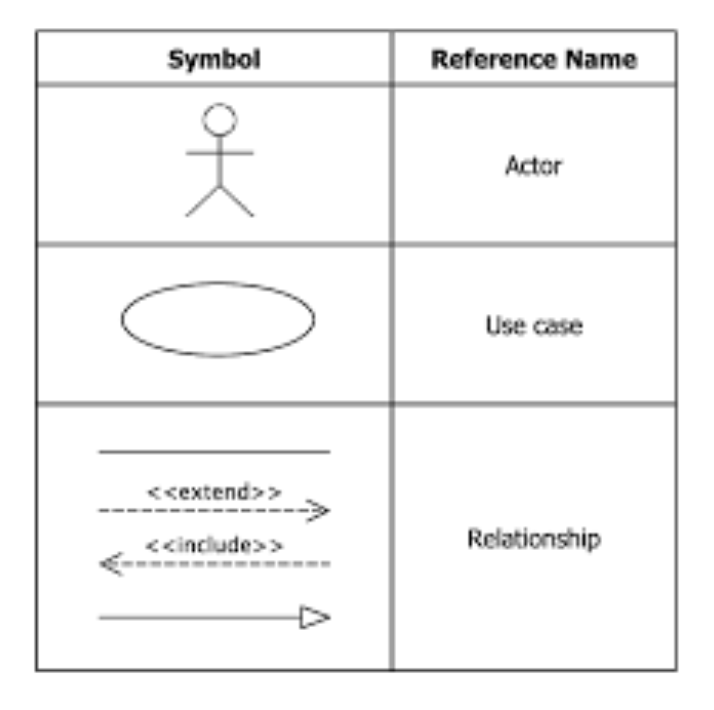
\includegraphics[scale=0.7]{ass3.png}
	\end{center}	
\end{enumerate}
\subsection{\textbf{Class Diagrams}}
\subsubsection{\textbf{What is a Class Diagram?}}
A class diagram is a static diagram that shows the structure of a system. It is a structural diagram that shows the
classes and their relationships in a system. It describes the attributes and operations of a class. It shows the static structure of a system.
\subsubsection{\textbf{What is the use of Class Diagram}}
\begin{enumerate}
	\item It is a graphical representation of the static structure of a system.
	\item It helps in understanding the structure of a system.
	\item It describes the classes and their relationships in a system.
	\item It is useful in identify the classes of a system.
	\item It is useful in identifying the relationships between the classes.
\end{enumerate}
\subsubsection{\textbf{Elements of a Class Diagram}}
\begin{enumerate}
	\item \textbf{Class:} A class is a set of objects that have similar attributes and operations. It is represented as a rectangle.
	\item \textbf{Attributes:} Attributes are the properties of a class. It is represented as a variable inside a class.
	\item \textbf{Operations:} Operations are the functions that can be performed on a class. It is represented as a function inside a class.
	\item \textbf{Relationships:} There are three types of relationships between classes:
	\begin{itemize}
		\item \textbf{Association:} Association is a relationship between two classes. It represents that the second class is a
		part of the first class. It is represented as a solid line between two classes.
		\item \textbf{Generalization:} Generalization is a relationship between two classes. It represents that the second class is a more specific version of the first class. It is represented as a solid line with an arrow pointing from the first class to the second class.
		\item \textbf{Dependency:} Dependency is a relationship between two classes. It represents that the second class is dependent on the first class. It is represented as a dashed line between two classes.
	\end{itemize}
	\begin{center}
		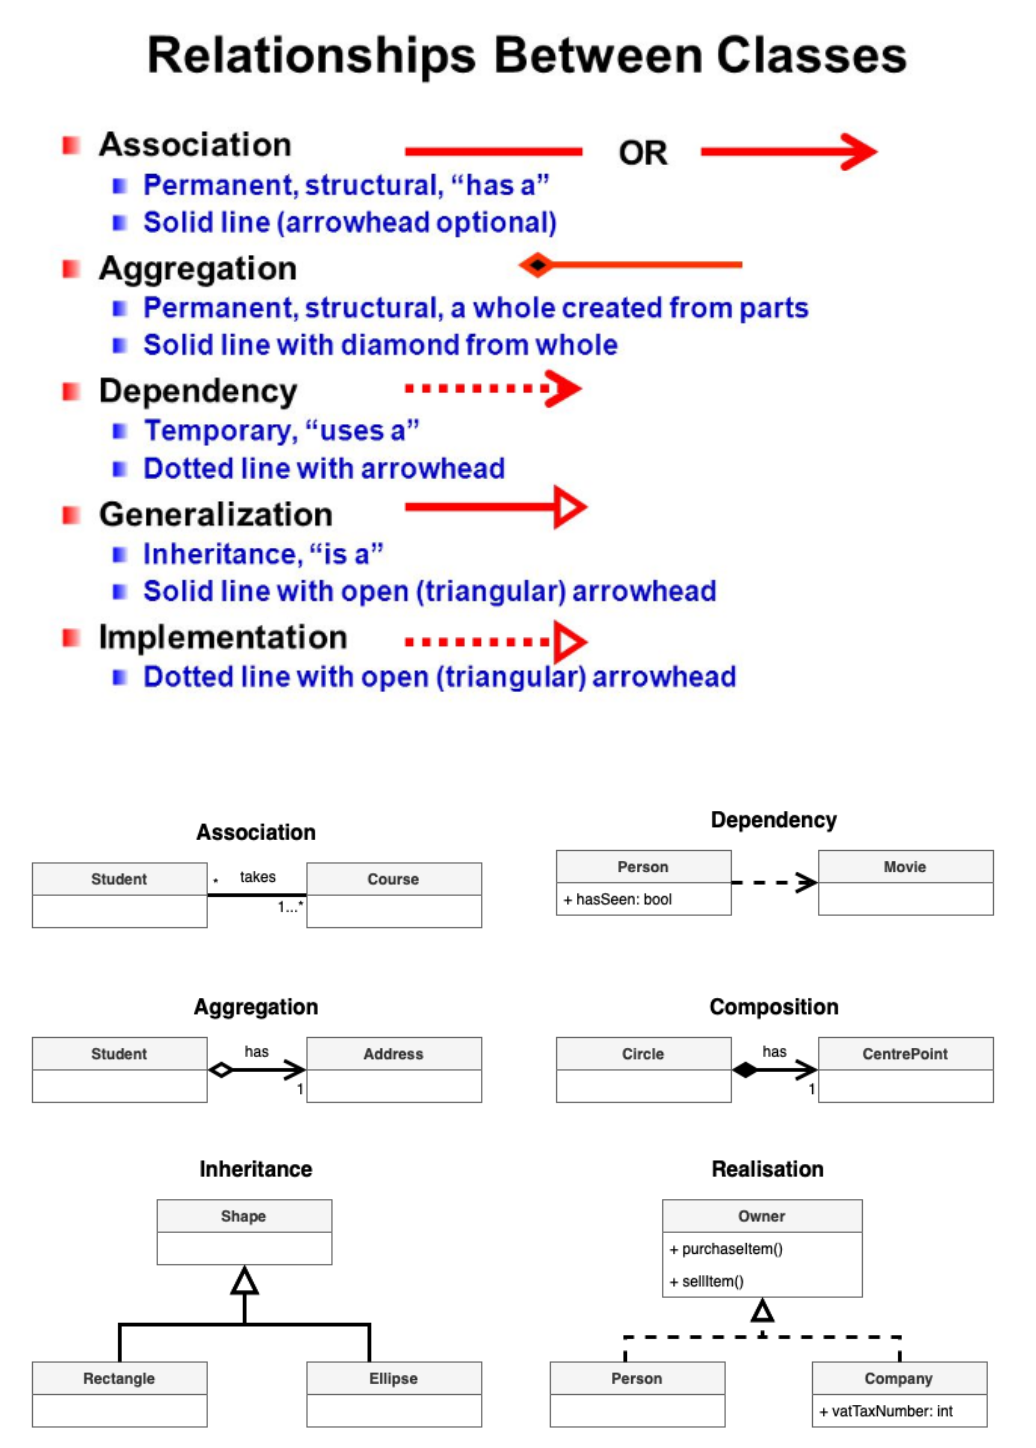
\includegraphics[scale=0.5]{asss3}
	\end{center}
\end{enumerate}
\section{\textbf{Procedure}}
\textbf{User Case Diagram}
\begin{itemize}
	\item Create Actors to represent classes of people, organizations, other systems, software or devices that interact with your system or subsystem.
	\item Create Use Cases for each of the goals that each actor seeks to achieve with the system.
	\item Use Associations to link actors to use cases.
	\item Use   \textless \textless include \textgreater \textgreater , \textless \textless extend \textgreater \textgreater and generalization to show the relationships among the use cases
\end{itemize}
\textbf{Class Diagram}
\begin{itemize}
	\item Write a problem statement, clearly defining the scope of the system.
	\item List out nouns as the probable classes from the problem statement.
	\item Draw the classes of the nouns focus should be on understanding relationships.
	\item Draw model of the system- the class and model. show the relationships between the classes.
	\item multiplicity in the class model. Data types not required.
\end{itemize}
\section{\textbf{Use Case Diagram:}}
\begin{center}
	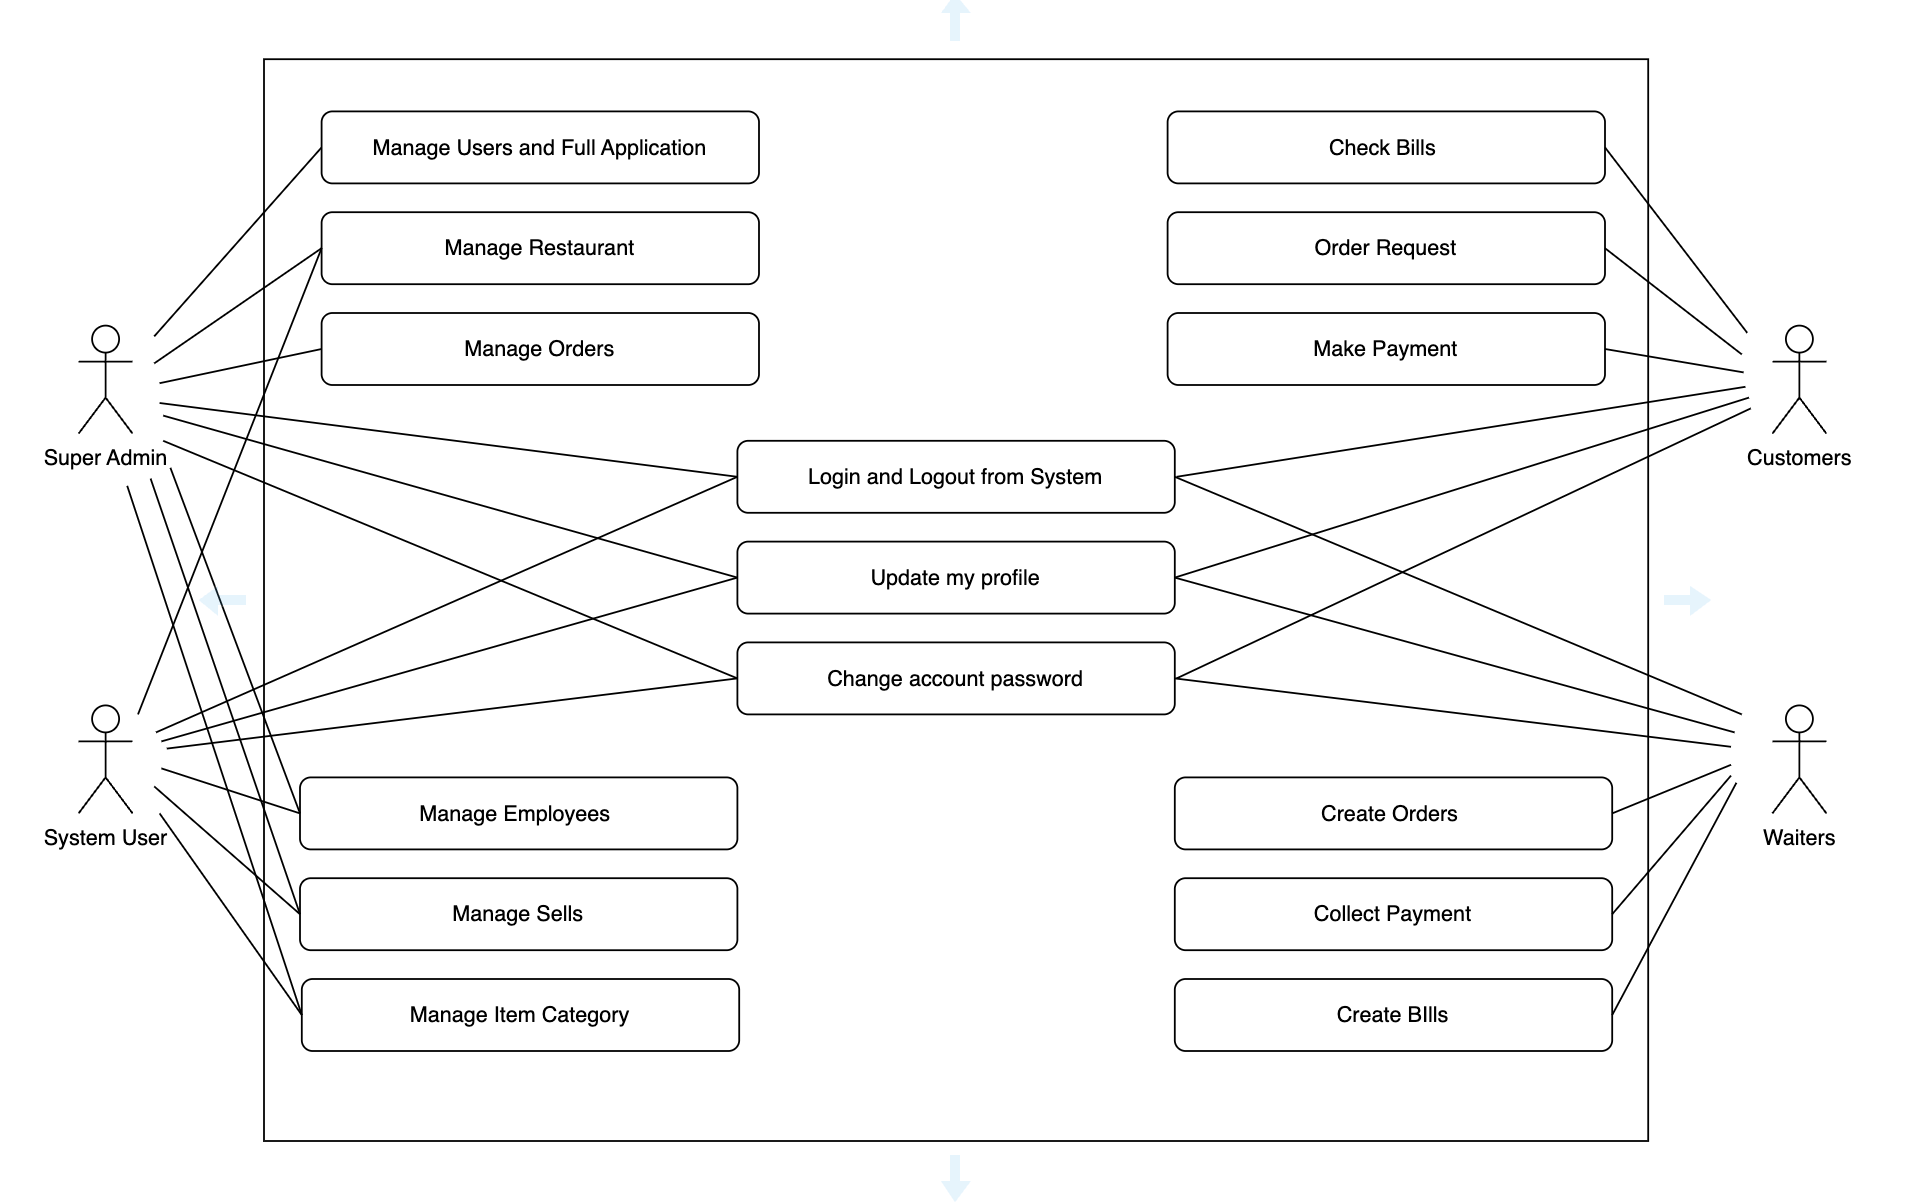
\includegraphics[scale=0.5]{usecasediagram}
\end{center}
\section{\textbf{Class Diagram}}
\begin{center}
	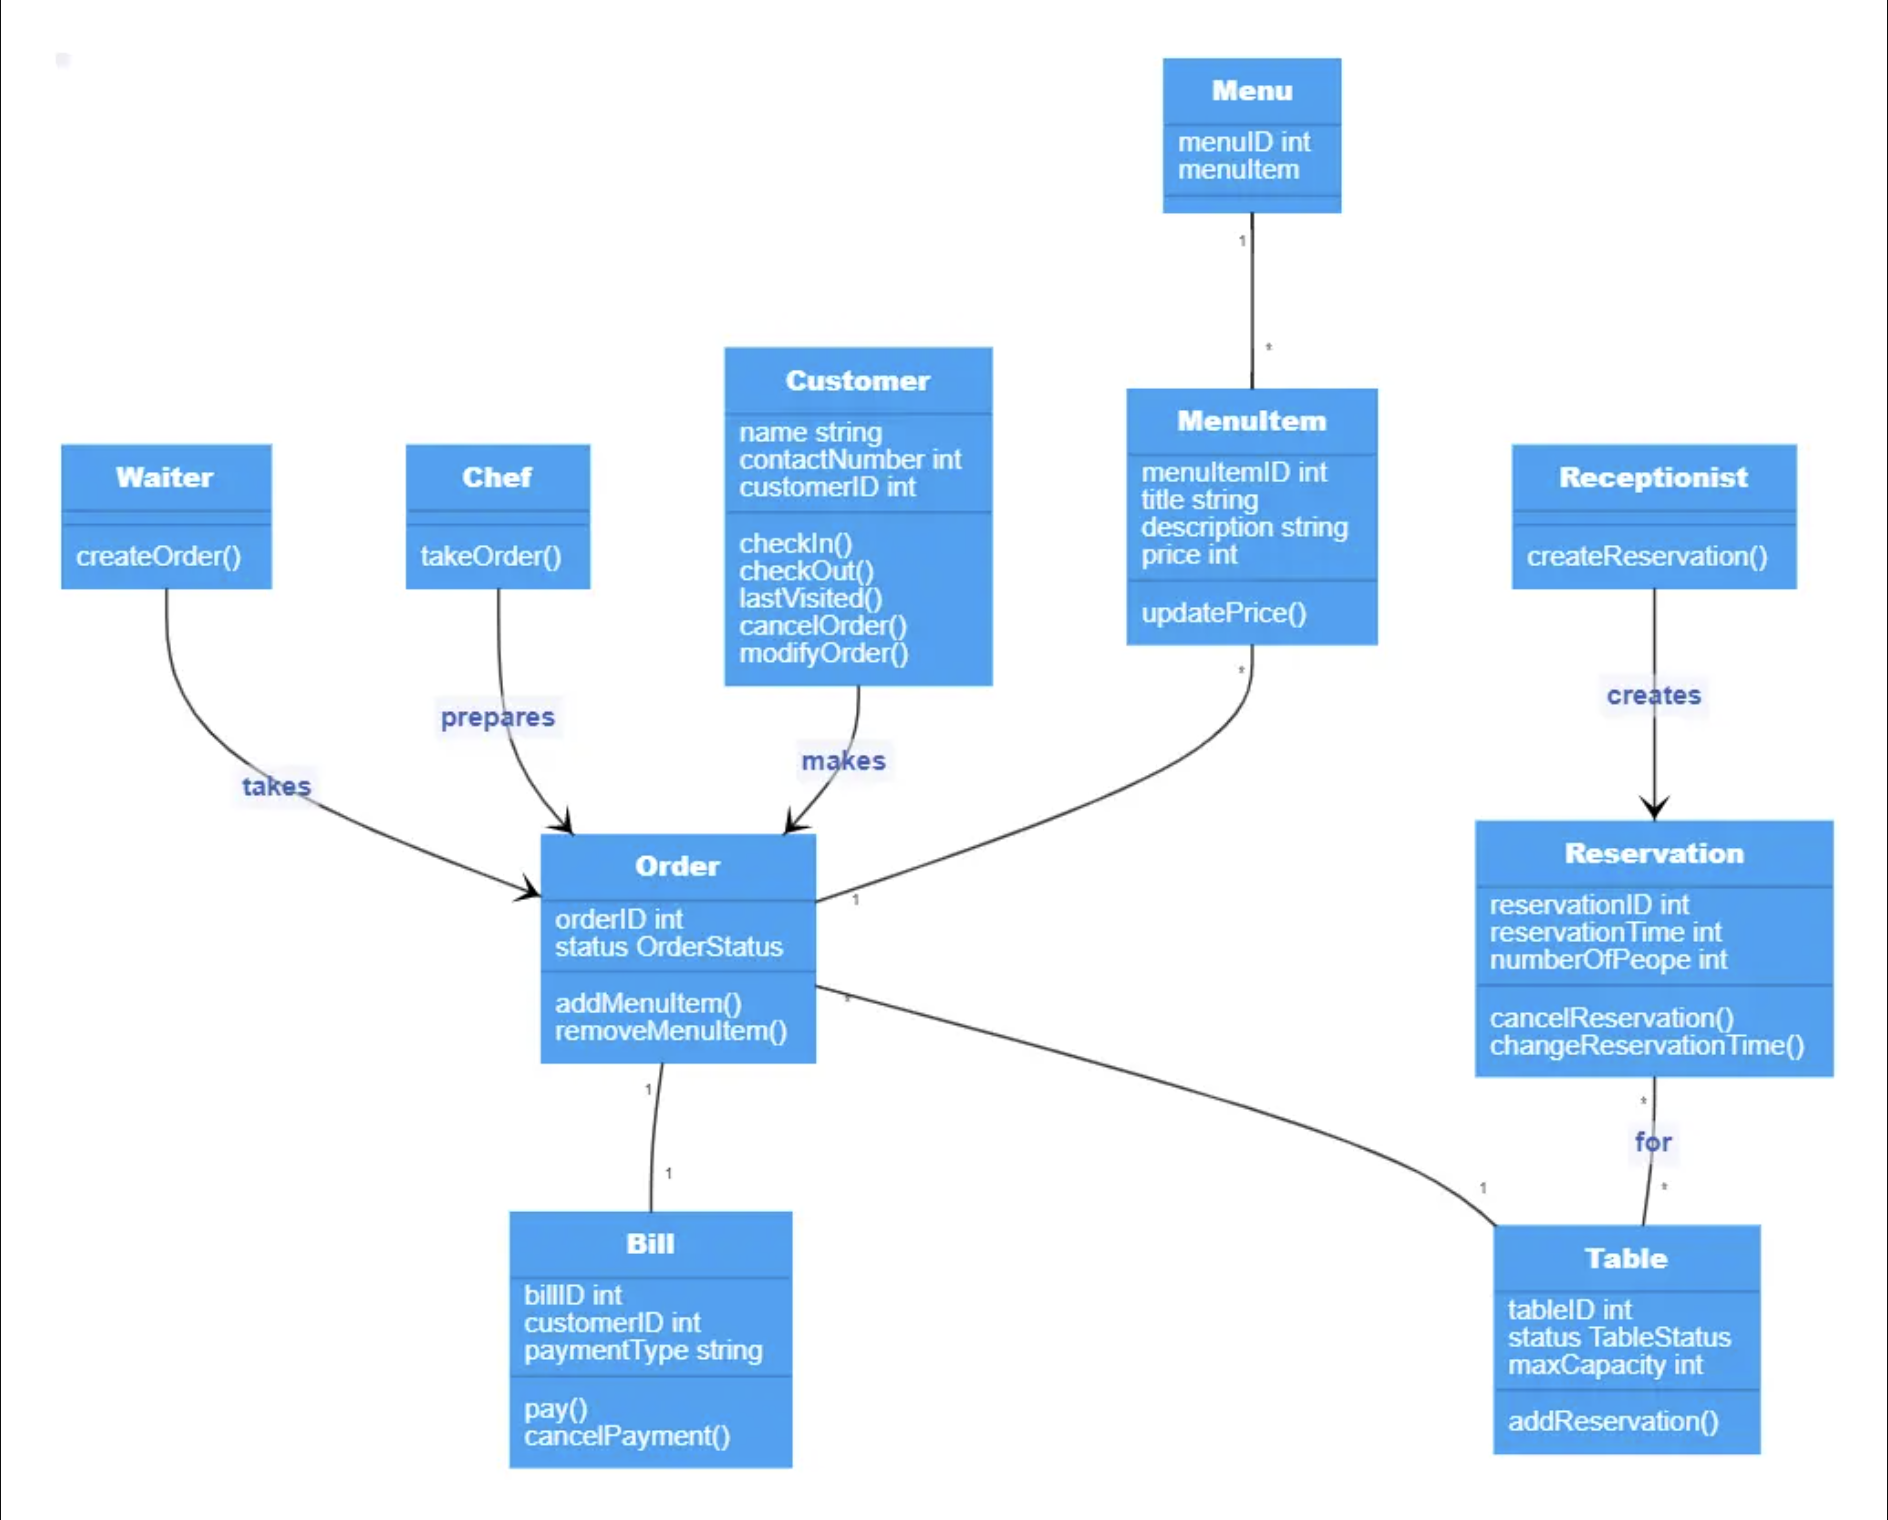
\includegraphics[scale=0.5]{casediagram}
\end{center}
\section{\textbf{Platform}}
Operating System:MacOS 64-bit\\
IDE:Visual Studio Code\\
External Program for Diagrams:Draw.io\\
\section{\textbf{Conclusion}}
Thus, we learnt about Use Case Diagrams and UML Class Diagrams in Detail.
\pagebreak
\section{\textbf{FAQ's}}
\subsection{What kind of relationships classes have? Explain all relationships with examples.}
\textbf{Ans.} There are several types of relationships between classes. Here are three main types of relationships:
\begin{enumerate}
	\item \textbf{Inheritance:} Inheritance is a relationship between two classes where one class (the child or derived class) inherits properties and behavior from another class (the parent or base class). This relationship is used to reuse code and to create a hierarchy of classes with increasing levels of specialization.\\
	\textbf{For Example:} Consider a class hierarchy for different types of vehicles in software. The base class could be "Vehicle" which has methods like "start" and "stop". The derived classes could be "Car", "Truck", and "Motorcycle", each inheriting the methods of the base class while also having their own unique methods.
	\item \textbf{Association:} Association is a relationship between two classes where one class uses an instance of another class. This is often referred to as a "has-a" relationship. This relationship is used to represent real-world relationships between objects.\\
	\textbf{For Example:} Consider a class for a Library Management System which has a relationship with a class for Books. The Library class might have a property called "books" which is an array of Book objects. This represents an association between the two classes, where the Library class "has-a" collection of Book objects.
	\item \textbf{Dependency:} Dependency is a relationship between two classes where one class depends on the other class. This means that changes to one class may affect the behavior of the other class.\\
	\textbf{For Example:} Consider a class for a Payment Gateway which depends on a class for Credit Card Validation. If the Credit Card Validation class changes its behavior, it may affect the behavior of the Payment Gateway class. This relationship is often represented by an arrow pointing from the dependent class to the independent class.
\end{enumerate}
\subsection{Explain any 2 terminologies used in Use case diagrams.}
\textbf{Ans.} Two terminologies used in Use Case Diagrams are:
\begin{enumerate}
	\item \textbf{Actor:} An actor is an external entity that interacts with the system. Actors are represented by stick figures in use case diagrams. They represent the roles played by people, systems, or devices that interact with the system being developed.\\
	\textbf{For Example:} Consider a use case diagram for an online shopping system. The customer and the system administrator are actors in this system. The customer interacts with the system to browse and purchase products, while the system administrator manages the products, orders, and user accounts.
	\item \textbf{Use Case:} A use case represents a specific functionality or behavior of the system. Use cases are represented by ovals in use case diagrams. They describe the actions that an actor can perform in the system.
	\textbf{For example:} In the online shopping system, a use case could be ``Browse Products'', ``Add to Cart'', ``Checkout'', ``Manage Products'', ``Manage Orders'', etc. Each of these use cases represents a specific behavior of the system that can be initiated by an actor.
\end{enumerate}
\subsection{Explain the aggregation and composition in diagram?}
\begin{enumerate}
	\item \textbf{Aggregation:} Aggregation is a relationship between two classes where one class is a part of another class. The part class can exist independently of the whole class, and can be part of other whole classes as well. The relationship is represented by a diamond shape on the side of the whole class, pointing to the part class.\\
	\textbf{For example} Consider a class hierarchy for a car manufacturing system. The Car class has an aggregation relationship with the Wheel class. The Wheel class can exist independently of the Car class and can be part of other classes, such as a Bicycle class. The Car class can also have a relationship with other part classes, such as the Engine class and the Seat class.
	\item \textbf{Composition:} Composition is a relationship between two classes where one class is made up of another class, and the part class cannot exist independently of the whole class. The whole class owns the part class and is responsible for its creation and destruction. The relationship is represented by a filled diamond shape on the side of the whole class, pointing to the part class.\\
	\textbf{For example} Consider a class hierarchy for a music player application. The MusicPlayer class has a composition relationship with the Playlist class. The Playlist class cannot exist without the MusicPlayer class, and is created and destroyed by the MusicPlayer class. The MusicPlayer class can have other part classes as well, such as the Song class and the User class, but the Playlist class is an essential part of the MusicPlayer class and cannot exist independently.
\end{enumerate}
\end{document}
